\documentclass{beamer} 
\usepackage{beamerthemesplit} 
\usepackage{wrapfig} 
\usepackage{verbatim} 
\usetheme{SPbGU} 
\usepackage{pdfpages} 
\usepackage{amsmath} 
\usepackage{cmap}
\usepackage{array} 
\usepackage[T2A]{fontenc} 
\usepackage[utf8]{inputenc} 
\usepackage{tikz} 
\usetikzlibrary{positioning, automata}
\usepackage{multirow} 
\usepackage[noend]{algpseudocode} 
\usepackage{algorithm} 
\usepackage{algorithmicx} 
\usetikzlibrary{shapes,arrows} 
\usepackage{fancyvrb} 
\usepackage{pgfplots} 
\usepackage{sidecap} 
\usepackage{soul}
\usepackage{xcolor}
\usepackage{tabu}
\usepackage{tikz}
\usetikzlibrary{calc}
\usepackage{zref-savepos}
\usepackage{colortbl}
\usepackage[normalem]{ulem}
\pgfplotsset{compat=1.9} 
\newtheorem{rutheorem}{Теорема} 
\newtheorem{ruproof}{Доказательство} 
\newtheorem{rudefinition}{Определение} 
\newtheorem{rulemma}{Лемма} 
\beamertemplatenavigationsymbolsempty 

\newcounter{NoTableEntry}
\renewcommand*{\theNoTableEntry}{NTE-\the\value{NoTableEntry}}

\newcommand*{\strike}[2]{%
	\multicolumn{1}{#1}{%
		\stepcounter{NoTableEntry}%
		\vadjust pre{\zsavepos{\theNoTableEntry t}}% top
		\vadjust{\zsavepos{\theNoTableEntry b}}% bottom
		\zsavepos{\theNoTableEntry l}% left
		\hspace{0pt plus 1filll}%
		#2% content
		\hspace{0pt plus 1filll}%
		\zsavepos{\theNoTableEntry r}% right
		\tikz[overlay]{%
			\draw
			let
			\n{llx}={\zposx{\theNoTableEntry l}sp-\zposx{\theNoTableEntry r}sp-\tabcolsep},
			\n{urx}={\tabcolsep},
			\n{lly}={\zposy{\theNoTableEntry b}sp-\zposy{\theNoTableEntry r}sp},
			\n{ury}={\zposy{\theNoTableEntry t}sp-\zposy{\theNoTableEntry r}sp}
			in
			(\n{llx}, \n{lly}) -- (\n{urx}, \n{ury})
			;
		}% 
	}%
}

\title[Effective CFL-reachability]{Уточнение сложностных оценок для задачи поиска путей с контекстно-свободными ограничениями} 
% То, что в квадратных скобках, отображается в левом нижнем углу. 
\institute[]{ JetBrains Research, Programming Languages and Tools Lab  \\
    СПбАУ, СПбГУ } 

\author[Екатерина Шеметова]{Екатерина Шеметова}

\date{14.12.2019} 

\begin{document} 
\definecolor{red}{RGB}{255,0,0} 

{
\begin{frame}[fragile]
  \begin{tabular}{p{2.0cm} p{4.5cm} p{1.5cm} p{1cm}}
   \begin{center}
      
\includegraphics[height=1.5cm]{pictures/jetbrainsResearch.pdf}
    \end{center}
    &
    \begin{center}
      
\includegraphics[height=1.5cm]{pictures/YC_logo.pdf}
    \end{center}
    &
    \begin{center}
      
\includegraphics[height=1.5cm]{pictures/au-logo-full.png}
    \end{center}
    &
    \begin{center}
      
\includegraphics[height=1.5cm]{pictures/SPbGU_Logo.png}
    \end{center}
  \end{tabular}
  \titlepage
\end{frame}
}


\begin{frame}
\frametitle{CFL-reachability (CFPQ)}
        \begin{center}
           достижимость в графе + контекстно-свободные ограничения
        \end{center}



\tikzset{every state/.style={minimum size=0pt}}
\begin{figure}[h]
    \centering        
    \begin{tikzpicture}[shorten >=1pt,auto, node distance=0.8cm]
       \node[state] (q_0)                      {$s$};
       \node[state] (q_1) [right=of q_0] {};
       \node[state] (q_2) [right=of q_1]       {};
       \node[state] (q_3) [right=of q_2]       {};
       \node[state] (q_4)   [right=of q_3]                    {};
       \node[state] (q_5) [right=of q_4] {};
       \node[state] (q_6) [right=of q_5]       {};
       \node[state] (q_7) [right=of q_6]       {$t$};
        \node[state] (q_8) [above=of q_2]       {};
        \node[state] (q_9) [above right=of q_8]       {};
       \node[state] (q_10) [below right=of q_9]       {};
        \path[->]
        (q_0) edge node {$[$} (q_1)
        (q_1) edge node {$($} (q_2)
        (q_2) edge node {$e$} (q_3)
        (q_3) edge node {$[$} (q_4)
        (q_4) edge node {$e$} (q_5)
        (q_5) edge node {$]$} (q_6)
        (q_6) edge node {$]$} (q_7)
        (q_4) edge[above] node {$]$} (q_10)
        (q_10) edge[above] node {$)$} (q_9)
        (q_9) edge[above] node {$e$} (q_8)
        (q_8) edge[left] node {$e$} (q_2);

    \end{tikzpicture}
\end{figure}
\centering
\textcolor{green}{[(e[])eee[e]]}


\begin{itemize}
\item Вход: контекстно-свободная грамматика $G$ и помеченный ориентированный граф $D$
\itemСферы применения: статический анализ кода, запросы к графовым базам данных, цепные запросы Datalog, ...
\end{itemize}
\end{frame}

\begin{frame}
\frametitle{Зачем изучать сложность задачи CFPQ? Мотивация}
\textbf{1. Разботка более эффективных алгоритмов}

 \centering                               
... хотя бы для частных случаев

\begin{itemize}
\item CFL-reachability решается за $O(n^3)$ ($n$ --- число вершин в графе)
\item С параллельными алгоритмами тоже всё плохо --- задача $P$-полная
\end{itemize}
\end{frame}

\begin{frame}
\frametitle{Зачем изучать сложность задачи CFPQ? Мотивация}
\textbf{2. ``Кубический барьер''}


 (Nevin Heintze and David McAllester, 1997): On the Cubic Bottleneck in Subtyping and Flow Analysis

Существует т.н. ``кубический барьер'' сложности различных задач анализа программ.
\\\textit{Открытая проблема:} существует ли алгоритм, работающий за $O(n^{3-\varepsilon})$ (т.н. \textit{субкубический алгоритм})?
\end{frame}

\begin{frame}
\frametitle{Подходы к решению}

Если всё так плохо, можно посмотреть на эффективные частные случаи
\begin{itemize}
\item Почему они эффективны?
\item Можно ли их обобщить?
\end{itemize}
\end{frame}


\begin{frame}
\frametitle{Частные случаи: параллельная сложность}
\begin{itemize}
\item Есть подклассы грамматик, для которых задача хорошо параллелится
\item Что объединяет эти эффективные классы? Много ли их? Почему они обладают этим свойством? Можем ли мы получить новые, полезные на практике?
\end{itemize}
\end{frame}

\begin{frame}
\frametitle{Частные случаи: параллельная сложность}
\begin{itemize}
\item Есть подклассы грамматик, для которых задача хорошо параллелится
\item Что объединяет эти эффективные классы? Много ли их? Почему они обладают этим свойством? Можем ли мы получить новые, полезные на практике?
\end{itemize}

\textbf{Результаты}
\begin{itemize}
\item Параллельная эффективность зависит от свойств автомата --- наличие ограничений на стек
\item Нашли большой класс таких языков: bounded-oscillation языки
\item Этот класс включает в себя большое количество ранее известных классов
\item Побочный эффект: возможно, этот класс ``разыскивает'' Datalog-сообщество
\end{itemize}
\end{frame}

\begin{frame}
\frametitle{Подходы к решению}

Сведение к другим задачам
\begin{itemize}
\item Сводим к известной задаче из другой области
\item Fine-grained complexity (мелкозернистая сложность)
\end{itemize}
\end{frame}

\begin{frame}
\frametitle{Сведение к инкрементальному транзитивному замыканию}
Свели CFL-reachability к инкрементальному транзитивному замыканию графа


\textbf{Результаты}
\begin{itemize}
\item Получили сложность $O(n^3/\log n)$
\item Ускорили алгоритм инкрементального ТЗ на логарифмический фактор
\item Получили интересные и эффективные частные случаи: планарные графы, графы с ограниченной степенью вершин и т.д.
\item Новые возможности в использовании идей из линейной алгебры
\end{itemize}
\end{frame}

\begin{frame}
\frametitle{Fine-grained complexity (мелкозернистая сложность)}
Новый раздел теории сложности, посвященный более точным оценкам сложности полиномиальных алгоримов


Согласно гипотезe OMv из мелкозернистой сложности, в общем случае ускорение инкрементального транзитивного замыкания получить сложно
\begin{figure}
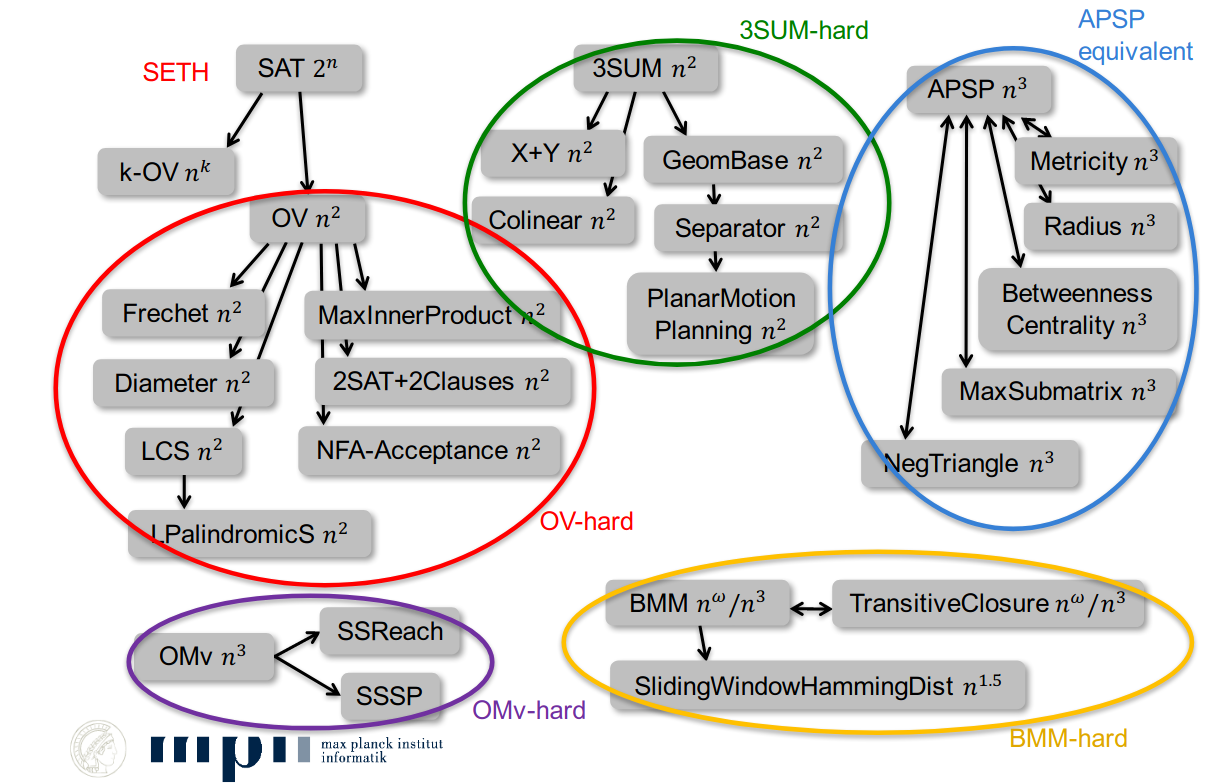
\includegraphics[scale=0.2]{pictures/hierarhy.png}
\end{figure}
\end{frame}

\begin{frame}
\frametitle{Публикации }
\begin{itemize}
\item Ekaterina Shemetova, Alexander Okhotin, Semyon Grigorev. Rational index of bounded-oscillation languages.
\\\textbf{ориентировочно журнал ``International Journal of Foundations of Computer Science''} 
\\\textit{Статус: подготовлена; думаем, куда подать}
\item Ekaterina Shemetova, Rustam Azimov, Egor Orachev, Ilya Epelbaum, Semyon Grigorev. One Algorithm to Evaluate Them All: Unified Linear Algebra Based Approach to Evaluate Both Regular and Context-Free Path Queries.
\\ \textbf{Журнал ``Information Systems Frontiers''}
\\\textit{Статус: подготовлена }
\end{itemize}
\end{frame}

\begin{frame}
\frametitle{Гранты, студенты}
\begin{itemize}
\item Грант РНФ под руководством Александра Охотина
\item Конкурс стипендий Президента для молодых учёных и аспирантов
\begin{itemize}
\item Уточнение сложностных оценок задачи поиска путей с ограничениями в терминах контекстно-свободных языков и разработка более эффективных алгоритмов для общего и частных случаев задачи
\item Заявка подана, находится на рассмотрении
\end{itemize}
\item Студенты: Александра Истомина (СПбГУ), Александра Олемская (НИУ ВШЭ), работают над частными случаями инкрементального транзитивного замыкания
\end{itemize}
\end{frame}

\begin{frame}
\frametitle{Планы и текущая работа}
\begin{itemize}
\item Продолжаем работу по параллельной сложности: на самом деле мы нашли гораздо больше классов с интересными свойствами
\item Углубляемся в fine-grained complexity: получение оценок исходя из гипотезы OMv
\item Изучение сводимости CFPQ к задачам из линейной алгебры и другим хорошим задачам
\item Дальнейшее рассмотрение частных случаев (классов графов и грамматик)
\item Логарифмическое ускорение CFPQ (это целое искусство)
\end{itemize}

\end{frame}
\end{document}

